\chapter{Numerical Dependencies in Database and Data Mining}\label{chap:numdep}

\section{Numerical Dependencies in Database Applications}


\subsection{Mining a relation for a set of NDs}

We consider only singleton right hand sides. For a relation $R$ with
$n$ attributes we have $n 2^{n-1}$ NDs returned by this algorithm.

\medskip

{\renewcommand{\baselinestretch}{1}
\begin{figure}[ht]
\fbox{
\begin{minipage}{16cm}
\begin{algorithm}[{\rm ND\_mine}($r$, $R$)]\label{alg:mine}
\begin{rm}
\begin{tabbing}
t1\=t2\=t3\=t4\=t5\=t6\=t7\=t8\=t9\= \kill \\
\ra.  \> \> {\bf begin} \\
\sa.  \> \> \> ND\_set := $\emptyset$;\\
\sa.  \> \> \> {\bf for each} $A \in R$ {\bf do}\\
\sa.  \> \> \> \> {\bf for each} $W \in \mathcal{P}$(R - A) {\bf do}\\
\sa.  \> \> \> \> \>  $max_k$ := 0; \\
\sa.  \> \> \> \> \>   {\bf for each} partition ${\cal B}$ of $r$ on
$W$ {\bf do}\\
\sa.  \> \> \> \> \> \>  k := The number of different $A$ values in ${\cal B}$; 
\\
\sa.  \> \> \>  \> \> \> {\bf if } k $> max_k$ {\bf then} \\
\sa.  \> \> \> \> \>\>   \>$max_k$ := k; \\
\sa. \> \> \> \> \> \>  {\bf end if}; \\
\sa.  \> \> \> \> \>  \> ND\_set := ND\_set $\cup$ $\{ W \to^{max_k} A \}$; \\
\sa. \> \> \>  \> \>  {\bf end for}; \\
\sa. \> \> \>  \>   {\bf end for}; \\
\sa. \> \> \>    {\bf end for}; \\
\sa. \> \> \> {\bf return} ND\_set;  \\
\sa. \> \> {\bf end.}
\end{tabbing}
\end{rm}
\end{algorithm}
\end{minipage}}
\end{figure}
}

\begin{itemize}
\item The computational complexity of this algorithm is O($n^2 2^{n-1}
\mid r \mid log \mid r \mid$)
\item Drop supersets of attributes? Restrict to singleton left and right
hand sides - O($n^3\mid r \mid log \mid r \mid$)
\item When the lhs of any ND is $\emptyset$ then the ND corresponds
directly to the domain size
\item The scale of the mining can be cut down by using axioms provided
in \cite{gm85b,gm85a} when exact details are not required for
dependencies of the form $W \to^k A$ where $W = YV$ and we already
know $Y \to^{k_1} A$ and $V \to^{k_2} A$ which would give $k \le K_1$
or $k \le k_2$, depending on the larger partition.
\end{itemize}
 

\section{The Chase Procedure for NDs}
\index{Chase Procedure!for NDs}

We now show how CHASE($r$, F) can be generalised to CHASE($r$, N), where N is
a set of NDs over R, shown in Figure~\ref{alg:ndchase}.

{\renewcommand{\baselinestretch}{1}
\begin{figure}[ht]
\fbox{\begin{minipage}{16cm}
\begin{algorithm}[{\rm CHASE}($r$, {\rm N})]\label{alg:ndchase}
\begin{rm}
\begin{tabbing}
t1\=t2\=t3\=t4\=t5\=t6\=t7\= \kill \\
\ra.  \> \> {\bf begin} \\
\sa.  \> \> \> Result := $r$; \\
\sa.  \> \> \> Tmp := $\emptyset$; \\
\sa.  \> \> \> {\bf while} Tmp $\not=$ Result {\bf do} \\
\sa.  \> \> \> \> Tmp := Result; \\
\sa.  \> \> \> \> {\bf if} $\exists X \to^k Y \in$ N, $\exists t_1, t_2, \ldots, t_k, t_{k+1} \in$ Result such that  \\
    \> \> \> \> \> $t_1$[X] = $t_2$[X] = $\ldots$ = $t_k$[X] = $t_{k+1}$[X] \\
    \> \> \> \> \> but $t_1$[Y] $\not=$ $t_2$[Y] $\not= \ldots \not=$ $t_k$[Y] $\not=$ $t_{k+1}$[Y] {\bf then} \\ 
\sa. \> \> \> \> \> {\bf for each} $A \in$ Y$-$X {\bf do} \\
\sa. \> \> \> \> \> \> \> $t_i$[A],$t_j$[A], := max($t_i$[A],$t_j$[A])
    for two distinct values $i,j \in 1,\ldots,k+1$; \\
\sa. \> \> \> \> \> {\bf end for} \\
\sa.  \> \> \> \> {\bf end if} \\
\sa.  \> \> \> {\bf end while} \\
\sa. \> \> \> {\bf return} Result;  \\
\sa. \> \> {\bf end.}
\end{tabbing}
\end{rm}
\end{algorithm}
\end{minipage}}
\end{figure}
}

We leave it to the reader to verify that when $k = 1$, i.e. X $\to^k$ Y is an
FD, then CHASE($r$, N) reduces to CHASE($r$, F).


\begin{lemma}\label{th:algterm}
\begin{rm}
Algorithm~\ref{alg:ndchase} terminates.
\end{rm}
\end{lemma}

{\em Proof.} No new values are introduced into the algorithm at any
time and therefore the algorithm must halt after executing the while
loop a finite number of times. $\Box$

\begin{theorem}\label{th:chase}
\begin{rm}
Given a set of NDs, N, then $\forall n \in N$, CHASE($r$,N) $\models n$.
\end{rm}
\end{theorem}

{\em Proof.} Direct from the definitions of the algorithm and of ND
satisfaction. $\Box$


\begin{itemize}
\item The axiom system given in \cite{gm85a} is shown to be sound and
complete in the special cases of either $|R| \le 3$ or the number of
NDs with $k > 1$ is at most one.
\item \cite{gm85b} shows that there is no finite sound and complete
axiomatisation for NDs. 
\end{itemize}






\section{ND Axiomatisation}


\subsection{Inferences for Numerical Dependencies}

\cite{gm85a} presents a set of sound inference rules for NDs. \cite{gm85b}
shows that there does not exist a {\em finite} set of sound and
complete inference rules for Numerical Dependencies.

\medskip
Rules 1-4 are as follows:
\begin{description}
\item[1] If $Y \subseteq X$ then infer $X \to Y$
\item[2] From $X \to^k Y$ infer $ZX \to^k ZY$
\item[3(a)] From $X \to^k Y$ and $Y \to^j Z$ infer $X \to^{k \cdot j} YZ$
\item[3(b)] From $X \to^k Y$ and $Y \to^j Z$ infer $X \to^{k \cdot j} Z$
\item[4] From $X \to^k Y$ infer $X \to^{k + 1} Y$
\end{description}

We now present another inference rule which generalises the rule
R5$_m$ of \cite{gm85b}, R6$_k$, which can be viewed as a generalised
transitivity rule for NDs wherein a bound on the number of attributes
required for inference is created based on the branching factor of the
NDs {\em and} the number of attributes on the left hand side of the FD
which determines attribute $Z$.

\smallskip
{\line
\begin{table}[ht]
\begin{tabular}{cl} \\
(R6$_{k,m}$): 	& from $\{ X \to^{k} Y_i \quad |  \quad 1 \le i \le \eta \} \cup 
		\{ Y_{i1}Y_{i2} \ldots Y_{im} \to Z   \quad |  \quad 1
		\le i1 < i2 < \ldots < im \le \eta \}$ \\ 
\rule{0cm}{5mm} & we can infer $X \to^{k} Z$ where $\eta =
		(m-1){k+1 \choose 2} + 1$\\
\end{tabular}
\end{table}}
\smallskip

\begin{theorem}\label{th:1}
\begin{rm}
Each rule R6$_{k}$ is sound and has minimal hypothesis.
\end{rm}
\end{theorem}

{\em Proof.} As for R5$_m$ in \cite{gm85b}, to be given. $\Box$

\medskip

We note that when $k$ = 1 then R6$_k$ reduces to transitivity of FDs,
and when $k$ = 2 then $\eta = 3m - 2$, the figure given in
\cite{gm85b}. 


\subsection{The Chase as an Inference Procedure}

We need to prove that the chase as an inference procedure for NDs can be shown
to be sound and complete. 

Given a set of NDs $N$ and an ND $\sigma$, we apply the chase as an
inference tool to discover if $N \models \sigma$. 
We create a relation $r_\sigma$ which for $\sigma = X \to^k
A$ has $k+1$ tuples with $k+1$ different values on attribute set $A$,
all values on X equivalent and all values in $R \backslash XA$ unique.

{\line
\begin{table}[ht]
\begin{center}
\begin{tabular}{c|c|c|c|c|c|} \cline{2-6}
 	& X 	& A 	& B$_1$ & $\ldots$ 	& B$_m$ \\ \cline{2-6}
$t_1$ 	& 1  	&  2  	& 1 	& $\ldots$ 	& 1 \\
$t_2$ 	& 1  	&  3  	& 2 	&  $\ldots$ 	& 2 \\
$\vdots$ & $\vdots$  &  $\vdots$  & $\vdots$ & $\ddots$ & $\vdots$ \\
$t_{k+1}$ & 1  &  $k+1$  & $k+1$ & $\ldots$ 	& $k+1$ \\ \cline{2-6}
\end{tabular}
\end{center}
\caption{\label{tbl:1.0} Relation to be chased by ND set N with
$\sigma = X \to^k A$, R $\backslash$ XA = $\{ B_1, \ldots, B_m \}$
and $m$ = $|$ R $\backslash$ XA $|$}
\end{table}}

Theorem~\ref{th:2} requires the notion of containment mapping.
For the definition we define a function $dom$ which returns the domain
of a relation.

\begin{definition}[Containment Mapping]\label{def:cm}
\begin{rm}
A containment mapping $\phi$ from $r_\sigma$ to a relation $r$ has
each value in $r_\sigma$ mapped by $\phi$ to a value in $dom$($r$).
This is extended to tuples over $R = A_1A_2 \ldots A_m$ as $\phi(t) =
\phi(t[A_1]),\phi(t[A_2]),\ldots, \phi(t[A_m])$ and extends to a
relation as $\phi(r) = \{ \phi(t) | t \in r \}$.
\end{rm}
\end{definition}

\begin{theorem}\label{th:2}
\begin{rm}
Given a set of Numerical Dependencies N and a ND $\sigma = X \to^k Y$,
N $\models \sigma$ iff $\neg\exists t^c_1[A] \not= t^c_2[A] \not= \ldots
\not= t^c_{k+1}[A]$ where $t^c_1,t^c_2,\ldots,t^c_{k+1} \in
r_\sigma^c$ and $r_\sigma^c$ = chase($r_\sigma$,N).
\end{rm}
\end{theorem}

{\em Proof.} (if) We assume that $Y \not\subseteq Z$. We let $r$ be a
relation over $R$ such that $r \models N$; we show that $r \models
\sigma$. Let $t_1, t_2, \ldots, t_{k+1} \in r$ such that $t_1[X] =
t_2[X] = \ldots = t_{k+1}[X]$. We claim that for some $i,
j \in \{1, 2, \ldots, {k+1}\}$ there exists $t_i[Y] = t_j[Y]$.

\smallskip
Let $\phi$ be a containment mapping from $r_\sigma$ to $r$ such that
$\phi(u_1) = t_1, \phi(u_2) = t_2, \ldots, \phi(u_{k+1}) = t_{k+1}$. We
shall prove that $\phi$ is additionally a containment mapping from
CHASE($r_\sigma$, N) to $r$ so that for some $i,j \in r_\sigma^c$,
$\phi(t_i^c[Y])$ = $\phi(t_j^c[Y])$ implies $t_i[Y] = t_j[Y]$.\\
\smallskip
We prove this by induction on the number of steps, $s$, required to compute
CHASE($r_\sigma$, N).\\

({\em Basis}):
If $s = 1$ then for some ND $W \to^k Z \in N$ two values are equated 
where $W \subseteq Z$ and $Y \subseteq Z$ and so therefore 
$t_i[Y] = t_j[Y]$ for some $i,j$.
\smallskip
 
({\em Induction}):
We assume that the result holds when $s$ steps of the chase procedure
are required. We now prove it to be true when $s+1$ chase steps are
required. We let the $s+1$ chase step be for an ND $W \to^k Z$ and
$w_i, w_j$ be two tuples in $r_\sigma$. The $s+1$ step either modifies
$w_i$ or $w_j$. For some subset $B \subseteq Z$ either $w_i[B]$ or
$w_j[B]$ is modified so that $w_i[B] = w_j[B] = t_i^c[Y] = t_j^c[Y]$.
Now, given $w_i[W] = w_j[W]$ then $\phi(w_i[W]) = \phi(w_j[W])$ by the
inductive hypothesis.  Therefore $\phi(t_i^c[Y]) = \phi(t_j^c[Y]) =
\phi(w_i[B]) = \phi(w_j[B]) = t_i[Y] = t_j[Y]$ holds given that $r
\models W \to^k Z$.\\

\smallskip

(only-if) If $\neg\exists t_i^c[Y] = t_j^c[Y]$ for some $i,j \in {1,2,
\ldots, k+1}$ then we can contruct a relation $r$ which satisfies all
$n \in N$ but but violates $\sigma$. \\

\smallskip
Alternatively, the chase for $r_\sigma$ can be shown to be isomorphic
to a relation $r$ which satisfies N by mapping each value in
$r_\sigma^c$ to a value in dom(r). $\Box$


\begin{theorem}\label{th:3}
\begin{rm}
The chase inference procedure for Numerical Dependencies is sound and complete.\end{rm}
\end{theorem}

{\em Proof.} Soundness of the chase as an inference procedure is
understood. Given a set of NDs N and an ND $\sigma = X \to^k A$ we
need to show completeness, ie. $N \models \sigma$ implies that $N
\vdash \sigma$. As for the proof procedure given in \cite{ll97c} we show
that the (if) part of Theorem~\ref{th:2} implies that $N \vdash
\sigma$. We show this by induction on the number of chase steps $s$
required to compute CHASE($r_\sigma$,N).

\smallskip
({\em Basis}):
If s = 1, then the chase procedure is applied once for some ND $W
\to^{k_2} Y$. This chase step equates two values in A and so $A \in Y$
 and $W \subseteq X$ (W must agree
on at least two tuples). Additionally $k_2 = k$ given that only one
chase step is required. We can infer $X \to^k Y$ by composition and $X
\to^k A$ by decomposition implying that $N \vdash \sigma$.
 
\smallskip
 
({\em Induction}):
Assume the result holds when the result of CHASE($r_\sigma$,N) takes 
$s$ steps. We prove that the result holds when the number of steps
required in $s+1$. The last chase step will apply to some ND $W \to^v Z
\in N$. For some $B \in Z$, two values $t_i[B]$ and $t_j[B]$,
initially distinct, will be equated.

\smallskip
If $B \not= A$ then we can assume that $N \vdash \sigma$ by the
 inductive hypothesis. We therefore assume that two values in A are
 equated in the $s+1$ step. We now consider the three cases that
 attribute set $W$
 may be related to attribute set $X$: \\

\begin{description}
\item[$W \subseteq X$] implies that we can infer $X \to^v A$ by
 composition. If $v > k$ then $v = k+1$ and no values will need to be
 equated in A, and so $v = k$. We infer that $N \vdash X \to^v A$ by
 decomposing $W \to^k Z$ to $W \to^k A$ and then apply the composition
 rule to obtain $X \to^k A$
\item[$W \supset X$] to be given
\item[$W$ is incomparable with $X$] to be given
\end{description} 
 $\Box$



\section{Data Mining with NDs}


\section{Dependency Mining Applications}\label{sec:fd_jobs}

Perhaps one of the prime applications for dependency mining is as a database
design tool which the database designer can use in conjunction with a possible
instance of the data to be stored within the database.  Inference upon this 
example set will then provide the designer with vital information as to possible
unknown dependencies that be satisfied in the relation. The approach of 
Bell and Brockhausen \cite{bb95} in making inferences from the verified and
invalid data dependencies is aimed at {\em supporting} the database
designer. \\

Approximation of the dependency set, possibly approximated using numerical
dependencies, on a large database in existence may reveal unknown information
in the form of these dependencies which may hold in the database.  

\begin{example}
\begin{rm}
In a patient database within a hospital every patient visit is independently stored
within a {\em patient} details relation and a {\em disease/sympton/treatment} relation. 
Given a numerical dependency specified $DISEASE \to^{10} SYMPTON$ stating
that a disease can have at most 10 symptons, it may however be approximated
that $ADDRESS \: \: \: PATIENT \to^{6} SYMPTON$ showing that at most
6 of the sympton can occur at the same location for a patient.
\end{rm}
\end{example}

\subsection{Approximating FDs}


\subsection{The Lattice Theory of NDs}




\begin{definition}[More functional set of NDs]\label{def:more}
\begin{rm}
A set of NDs $N_1$ over R is {\em more functional} than a set of NDs 
$N_2$ over R, denoted by $N_2 \sqsubseteq N_1$, whenever
X $\to^{k_2}$ Y $\in N_2$ if and only if X $\to^{k_1}$ Y $\in N_1$ and 
$k_1 \le k_2$. 
\end{rm}
\end{definition}
\medskip

The set-theoretic relation, more functional than, 
is a partial order in the sets of NDs.
Assume that we are considering only sets of NDs over schema R which are more functional 
than a given set of NDs, N over R, each of the form X $\to^k$ Y, 
for some $k \ge 1$.
Then the family of sets of NDs that are more functional than N form a lattice
whose bottom element is N and whose top element is the set of FDs
induced by N, i.e. \{X $\to$ Y $\mid$ X $\to^k$ Y $\in$ N\}.
The {\em least upper bound}, $lub$, of $N_1$ and $N_2$ is the set of NDs
\{X $\to^{min(k_1, k_2)}$ Y $\mid$
X $\to^{k_1}$ Y $\in N_1$ and X $\to^{k_2}$ Y $\in N_2$\},
where $min(k_1, k_2)$ is the minimum of $k_1$ and $k_2$, and the 
{\em greatest lower bound}, $glb$, of $N_1$ and $N_2$ is defined similarly using maximum.
We call the lattice, whose top element is the set of FDs F over R
and whose bottom element is the set of NDs
\{X $\to^m$ Y $\mid$ X $\to$ Y $\in$ F\}, ${\cal L}_m$(F)
(or simply ${\cal L}_m$ if F is understood from context), with $m \ge 1$.


Therefore, we can {\em approximate} a set of FDs F by a set of NDs N
such that N $\sqsubseteq$ F. 
The {\em closer} N is to F in ${\cal L}_m$ the better the approximation is.
From now on we let ${\cal L}_m$ 
{\em be the lattice of NDs whose top element is} F
and assume that $\mid r \mid = m+1$, with $m \ge 1$.

\medskip

\begin{definition}[Maximal a set of NDs]
\begin{rm}
The {\em maximal} set of NDs of $r$ with respect to F,
denoted by $maximal(r$, F), is the maximal set N of NDs
in ${\cal L}_m$(F) (with respect to $\sqsubseteq$) such that $r \models$ N.
\end{rm}
\end{definition}
\medskip

Given $r$ and F, $maximal(r$, F) can be computed in polynomial time in the
sizes of $r$ and F by a straightforward hill climbing procedure
on ${\cal L}_m$(F). For each X $\to$ A $\in$ F this procedure finds 
the minimal $k$ such that $r \models$ X $\to^k$ A, starting 
from X $\to^m$ A which $r$ trivially satisfies since $\mid r \mid = m$. 


\begin{definition}[Improvement set of a set of NDs]
\begin{rm}
The {\em improvement set} of $r$ with respect to F, 
denoted by $\mu$($r$, F), is defined as 
\begin{displaymath}
\mu(r, {\rm F}) = \{{\rm X} \to^k {\rm A} \mid 
{\rm X} \to^k {\rm A} \in maximal(r, {\rm F}) \mbox{ and }  k > 1\}.
\end{displaymath}
\end{rm}
\end{definition}
\medskip


{\renewcommand{\baselinestretch}{1}
\begin{figure}[ht]
\begin{center}
\fbox{\begin{minipage}{16cm}
\begin{algorithm}[{\rm MU}($r$, {\rm F})]\label{alg:mu}
\begin{rm}
\begin{tabbing}
t1\=t2\=t3\=t4\=t5\= \kill \\
1.  \> \> {\bf begin} \\
2.  \> \> \> m := $\mid r \mid$; \\
3.  \> \> \> N := the bottom element of $\mathcal{L}_m$ (F); \\
4.  \> \> \> {\bf while} $\exists$ G such that N $\cover$ G {\em and} $r \models$ G  {\bf do} \\
5.  \> \> \> \> N := G; \\
6.  \> \> \>  {\bf end while} \\
7.  \> \> \> \> N := $ \{X \to^k Y \mid X \to^k Y \in N $ {\em and} $k > 1 \} $ \\
8. \> \> \> {\bf return} N;  \\
9. \> \> {\bf end.}
\end{tabbing}
\end{rm}
\end{algorithm}
\end{minipage}}
\end{center}
\end{figure}
}



We introduce a measure for calculating the proximity of two ND sets using
their position within the lattice.  We show that this measure is a distance
function, satisfying reflexivity and symmetry, and is also a metric, 
satisfying the triangle inequality. Firstly, we begin by defining the best
approximation given by a set of NDs to their functional counterparts.
We define the {\em size} of a set of NDs N to be the number of attributes 
appearing in N including repetitions and define a {\em step}, either up
or down, to be exactly minus or plus one, respectively, to a single branch of
one ND within an ND set. Furthermore, we say that $N_2$ is {\em covered by} $N_1$, denoted by $N_2$ $\cover$ $N_1$, where $N_1, N_2 \in {\cal L}_m$, 
if $N_1 \not= N_2$, $N_2 \sqsubseteq N_1$ and
$\forall N^\prime \in {\cal L}_m$ such that 
$N_2 \sqsubseteq N^\prime \sqsubseteq N_1$ we have $N^\prime = N_2$.


\begin{definition}[The best approximation of a set of FDs]\label{def:best}
\begin{rm}
A set of NDs N over R is the {\em best approximation} of 
a set of FDs F over R with respect to a relation $r$ over R,
with $\mid r \mid = m+1$ (or simply the best approximation of F
if $r$ is understood from context), if $r \weak$ N 
and there does not exist a set of NDs, $N^\prime \in {\cal L}_m$
such that N $\cover$ $N^\prime$ and $r \weak N^\prime$.
\end{rm}
\end{definition}



\begin{proposition}[The number of NDs higher in the Lattice]
\begin{rm}
Given an ND set $N$ = \linebreak[4]   $\{ X_1 \to^{k_1} A_1, X_2 \to^{k_2} A_2,
 \ldots, X_n \to^{k_n} A_n \}$, the number of ND sets above this set in the
lattice is ($k_1 \cdot k_2 \cdot \ldots \cdot k_n$) - 1.
\end{rm}
\end{proposition}

{\em Proof.} An ND is higher in the lattice if within a 
set of NDs none of the $k_i$ branches have any values higher than
any of those in the set {\bf and} at least one of the NDs has some 
$k_j$ branch value
lower than one of those in the set. Each ND $X_i \to^{k_i} A_i$ within
the set can take $k_i$ values. We consider all permutations of these
values to get $k_1 \cdot k_2 \cdot \ldots \cdot k_n$ from which we 
must ensure that the ND set values of $N$ itself is not included to get
$k_1 \cdot k_2 \cdot \ldots \cdot k_n$ - 1. $\Box$

\smallskip

This provides us with the basis for a distance measure between an ND set
and its functional representation. However,  using this technique allows,
in some instances, ND sets which are the same number of steps below the
FD equivalent to have different values. This is due to ND sets containing
FDs or NDs which are close to being functional having less sets above them
in the lattice. To illustrate, if we have two ND sets $N_1,N_2$ each containing two NDs such that $N_1$ has dependencies with 4 and 2 as branches whilst $N_2$ has dependencies with 3 and 3 as branches then $N_1$ will have fewer ND sets
above it in the lattice though both are the same number of steps from their
functional equivalent, shown in Figure~\ref{latt:1}. We now introduce the 
metric we used in our simulations
and note that if we are interested in comparing ND sets with either more 
or less {\em near} FDs we can refer to the above measure 
whenever the metric provides the same distance.
\smallskip

In the following definition {\em distance} is defined as the number of
{\em steps} in the lattice. Definition~\ref{def:pfd} is used within
the simulations we conducted.

\begin{definition}[Proximity between two ND sets]
\begin{rm}
Given two sets of NDs $N_1$ and $N_2$ we define the metric as follows: 
\[
p(N_1,N_2) = \frac{\Sigma_{i = 1, 2} \mbox{ Distance from } N_i \mbox{ to }  lub \{ N_1, N_2 \}}
{\mbox{Maximum distance between any two ND sets to their $lub$ in the lattice}}
\]
\end{rm}
\end{definition}

\begin{definition}[Proximity to an FD set]\label{def:pfd}
\begin{rm}
Given a sets of NDs $N_1$ and a set of FDs $F$ which $N_1$ approximates
then the proximity between the two dependency sets is given by $p(N_1,F)$.
\end{rm}
\end{definition}

We define the bottom of the
lattice to be the set of NDs with each branching factor equivalent to
the domain size of the attribute on the right hand side of each
ND.

\smallskip
\begin{proposition}
\begin{rm}
The maximum distance between any two points in
the lattice to their $lub$ is always equivalent to the
distance from the bottom to the top of the lattice. 
\end{rm}
\end{proposition}

{\em Proof}. We prove this by induction on the NDs within the two ND sets.\newline 
\smallskip
\indent ({\em Basis}): We see that if $N_1$ and $N_2$ are empty then the
result is immediate.

\smallskip

({\em Induction}): We have two ND sets $N_1$ and $N_2$ which are distance
$d$ apart where $d \le m$ and $m$ is the maximum distance apart between
any two ND sets. We add an ND $X \to^{k_1} Y$
to $N_1$ and $X \to^{k_2} Y$ to $N_2$ which differ only
on their branching factor. Without loss of generality, if $k_1 < k_2$ then the
distance apart between $N_1$ and $N_2$ becomes $d + k_2 - k_1$. This 
remains less than or equal to the maximum distance apart which is $m + k'_2 -
k'_1$ where, without loss of generality, $k'_1 = 1$ (it is an FD) and
$k'_2$ is at the bottom of the lattice. $\Box$

\smallskip

The metric $p$ is a distance function given that the distance
between two NDs is zero only when they are equivalent and that 
$p(n_1,n_2) = p(n_2,n_1)$ always holds. It also satisfies the 
triangle inequality, whose proof we now outline. 

\begin{theorem}
\begin{rm}
Given three ND sets, $N_1$, $N_2$, and $N_3$, $p(N_1,N_2) + p(N_2,N_3)
\ge p(N_1,N_3)$.
\end{rm}
\end{theorem}
\smallskip

{\em Proof.} We show that if $N_1$, $N_2$ and $N_3$ are non-empty and the 
triangle
inequality holds then the addition of a new ND to each set which may
differ only on its branching factor will still satisfy the triangle inequality.
Assume we add three NDs $X \to^{k_i} A$ with $i = 1,2,3$ to $N_1,N_2$ and
$N_3$, respectively. We also assume, without loss of generality, that 
$k_1 < k_3$. We denote each ND set $N_i \cup \{ X \to^{k_i} A \}$ by $N'_i$
for $i = 1,2,3$. We perform induction on the NDs in each set.

\smallskip
({\em Basis}): If $N_1$ = $N_2$ = $N_3$ = $\emptyset$ then the 
result is immediate.

\smallskip
({\em Induction}):
 We assume that $k_2 \le k_1$, then $p(N'_1,N'_2)$ =
distance from $N_1$ to $lub(N_1,N_2)$ + distance from $N_2$ to $lub(N_1,N_2)$ +
$k_2 - k_1$. Similarly for $p(N'_2,N'_3)$ and $p(N'_1,N'_3)$ we have the
additional components, $k_3 - k_2$ and $k_3 - k_1$. Therefore, we have
$p(N'_1,N'_2) + p(N'_2,N'_3)$ = $p(N_1,N_2) + k_1 - k_2 + p(N_2,N_3) +
k_3 - k_2$ and $p(N'_1,N'_3)$ = $p(N_1,N_3) + k_3 - k_1$. We know that  
$p(N_1,N_2) + p(N_2,N_3) \ge p(N_1,N_3)$ holds and we see
 that  $k_1 - k_2 + k_3 - k_2 \ge k_3 - k_1$ holds if $k_1 \ge k_2$ which
is true, based on our initial assumption. We can similarly prove the 
triangle inequality for the case when $k_1 \le k_2$. $\Box$



\subsection{Partitioning a Relation for Average NDs}

\subsection{Similarity Measures and Numerical Depdencies}


\section{Evolving Example Relations to Satisfy FDs}
\index{Evolutionary Algorithm}



Example relations satisfying a given set of integrity constraints such as 
functional dependencies (FDs) are important during the database design 
activity in order to guide the designer towards the specification of a correct 
set of constraints for the application in hand \cite{sm81}. 

\smallskip

If the example relation shown to the database designer is too large then 
the designer will {\em not} be able to assimilate all the knowledge embedded in
that relation. Thus it would be useful to be able to generate random examples 
relations that satisfy F and whose maximal cardinality is specified by the 
database designer; in general, such an example may not be an Armstrong relation.
Moreover, it would also be useful to generate small random 
counterexample relations for FDs not logically implied by F; 
we note that for any FD that is not logically implied by F, 
a counterexample of two tuples can always be generated \cite{bdfs84}.
Both examples and counterexamples are important:
examples give the database designer an idea of what the actual 
data may look like, while counterexamples highlight FDs which 
may be violated and thus must be as compact as possible.

\smallskip

We propose that example and counterexample relations satisfy 
the following three requirements:
\begin{enumerate}
\item All example and counterexample relations will satisfy F.
\item The maximal cardinality of example relations will be 
specified by the database designer.
\item The cardinality of all counterexample relations will be two.
\end{enumerate}

It follows that as more example and counterexample relations are presented to
the database designer, FDs which are logical consequences of F are positively 
reinforced while FDs which are not logical consequences of F are negatively 
reinforced. (We observe that an example relation may also serve as a
counterexample relation for one or more FDs, but the database designer may
 prefer to view counterexamples separately.)
Another way of stating this reinforcement is that after a sufficient 
number of examples and counterexamples have been presented to the database 
designer, the intersection of the sets of FDs satisfied by these 
example and counterexample relations is exactly equivalent to F.

\smallskip

We say that a set of relations is {\em almost Armstrong} for F
if the intersection of the sets of FDs satisfied by this set of relations 
is equivalent to F. Our proposal is to replace the property of being an 
Armstrong relation by the property that a sufficient number
of examples and counterexamples in a set of such relations
 is almost Armstrong for F; indeed it may often be the case that an
example is itself an Armstrong relation and no explicit
counterexamples are required.

\smallskip

Our algorithm is evolutionary in that it incorporates a stochastic approach
for altering a relation by a {\em mutation} operation.
 The algorithm proceeds as
follows; initially a relation is randomly generated following
the input of the designer and a given FD set. This relation is then
 mutated based on a probabilistic selection of an unsatisfied FD  from the
given set and an attribute which assists violation of this FD in the relation.
We use numerical dependencies (NDs) \cite{gm85a,gm85b} as an
approximation of the unsatisfied FDs in the relation. 
The mutations steer the relation
towards a final state wherein all of the FDs in the specified set are
satisfied. It is a simple algorithm, and indeed a basic tenet 
of evolutionary programming is to create algorithms 
which do not constrain evolution too severely,
 much like organic evolution \cite{bs93}. All evolved relations are then mined 
using a quality function whose criterion is exact satisfaction of the given FD set. Example relations using NDs to approximate FDs together
with quality functions for assessing the discovered knowledge 
can be used as the basis for many dependency data mining algorithms \cite{kdd96}.

\smallskip

A deterministic approach used to generate an Armstrong relation
(Algorithm 14.2, \cite{Mann92}) has the severe drawback
 in that the same relation
is generated every time the algorithm runs.  Our probabilistic
approach is advantageous in that different example relations may
be generated from equivalent domain sizes and the tuple size may be
increased or decreased by the designer as desired. Moreover, as long as 
the number of tuples exceed the minimum size required for an Armstrong relation
 \cite{bdfs84,mr86} then one may
be returned.  Below this number and a deterministic approach fails
 whereas our evolutionary approach complies with the desires of the user
and returns a relation which, if selected from a batch or {\em 
population} of evolutions, is likely to be as high a quality
as possible given the domain and tuple restriction.  From the user's
point of view it may often be highly beneficial to examine a smaller
relation of a high quality, but less than one, as opposed to a larger Armstrong
relation (with a quality of one). To illustrate some
features of the evolutionary process we now present an example.

\begin{example}
\begin{rm}
For the schema $R$ containing attributes TEACHER, HOUR, and ROOM
we impose the FD TEACHER HOUR $\to$ ROOM, implying that no teacher
can be give a class in more than one room at the same time.
 We denote TEACHER, HOUR, and ROOM by $T, H$ and $R$,
 respectively, and show a deterministic
generated Armstrong relation (AR) in Table~\ref{tab:thr1}, an evolved 
Armstrong relation in Table~\ref{tab:thr2} (with an equivalent domain and one
less tuple), an evolved relation in Table~\ref{tab:thr3} with three
tuples depicting the best attainable quality (0.5) for the FD in a relation
of this size, and in Table~\ref{tab:thr4} we provide a counterexample
relation for the FD ROOM $\to$ HOUR which implies that a room can only ever be 
used at one time whilst satisfying our original specified FD.
\end{rm}
\end{example}

{\line
\begin{table}[ht]
\begin{minipage}[b]{8cm}
\begin{center}
\begin{tabular}{|c|c|c|} \hline
 T & H & R \\ \hline
 0 & 0 & 0 \\
 1 & 0 & 0 \\
 1 & 1 & 0 \\
 2 & 1 & 1 \\
 2 & 2 & 2 \\  \hline
\end{tabular}
\end{center}
\caption{\label{tab:thr1}Deterministic AR}
\end{minipage}
\hfill
\begin{minipage}[b]{8cm}
\begin{center}
\begin{tabular}{|c|c|c|} \hline
 T & H & R \\ \hline
 2 & 1 & 3 \\
 2 & 3 & 3 \\
 3 & 1 & 3 \\
 3 & 3 & 1 \\  \hline
\end{tabular}
\end{center}
\caption{\label{tab:thr2} Evolved AR}
\end{minipage}
\end{table}
\begin{table}[ht]
\begin{minipage}[b]{8cm}
\begin{center}
\begin{tabular}{|c|c|c|} \hline
 T & H & R \\ \hline
 2 & 0 & 1 \\
 2 & 2 & 0 \\
 0 & 2 & 0 \\ \hline
\end{tabular}
\end{center}
\caption{\label{tab:thr3} Evolved example relation}
\end{minipage}
\hfill
\begin{minipage}[b]{8cm}
\begin{center}
\begin{tabular}{|c|c|c|} \hline
 T & H & R \\ \hline
 1 & 1 & 0 \\
 0 & 0 & 0 \\ \hline
\end{tabular}
\end{center}
\caption{\label{tab:thr4} Counterexample relation}
\end{minipage}
\end{table}
}

In order to test the viability of our approach we conducted simulations
over 72 carefully chosen sets of FDs. 
 Each FD set was evaluated with respect to the average length of the
 evolution process and the final quality of the relations
 produced in batches
containing 1,000 runs, a single run being the process of mutating
a randomly generated relation until the given FD set is satisfied.
This was performed for around 80 batches, varying over domain and tuple
size which were both held constant within a batch. The domain and tuple
sizes each ranged on average from about one 
half to double the number of tuples required for a deterministic
Armstrong relation (based upon the specified FD example set).  The simulations
emphasised the validity of this approach within database
design, showing that many varying relations can be efficiently
evolved for an FD set with numerous domain and tuple inputs.
 They also showed that it is extremely useful to know the quality of an
 example relation, and additionally that Armstrong
relations are often formed within a batch. 




\section{Motivation}

\index{Randomised Algorithm}
\section{Mutating relations}
\label{sec:mutate}

Herein, we present an algorithm for {\em mutating} a relation.
Informally, given a relation which does not satisfy F, MUTATE($r$, F) 
randomly selects an ND, say X $\to^k$ A, in the improvement set of $r$ and 
stochastically modifies some of the tuple values in $r$.
We then define the syntactic property of non-interfering NDs 
and show that if the selected ND and another ND
Y $\to^g$ C in $maximal(r$, F) are non-interfering then, after the mutation, 
$r$ will still satisfy Y $\to^g$ C.
The non-interference property is important,
since if we evolve a relation to satisfy a set of FDs by iterating the
mutation operation, then the evolution process will be more efficient 
when the NDs in $maximal(r$, F) are non-interfering.

\medskip

The {\em mutation} of a relation over R with respect to a set of FDs over R 
denoted by MUTATE($r$, F), is defined as the relation resulting from invoking 
Algorithm~\ref{alg:mutate} presented below. In this algorithm we use LHS
 to denote the left hand side of an ND and RHS to denote the right hand
side.  This random selection of a side removes any bias which might otherwise
have been incurred if the selection of an attribute to mutate were
taken over the whole ND, given that the left hand side may be any
length less than or equal to $\mid R \mid$ but the right hand side is always singleton.


{\line
\begin{figure}[ht]
\begin{center}
\fbox{\begin{minipage}{16cm}
\begin{algorithm}[{\rm MUTATE}($r$, {\rm F})]\label{alg:mutate}
\begin{rm}
\begin{tabbing}
t1\=t2\=t3\=t4\=t5\= \kill \\
1. \> \>{\bf begin}\\
2. \>\> \> Result := $r$;\\
3. \>   \>\> Uniformly randomly select an ND $X \to^k A \in$ MU($r$,F);\\
4. \>   \>\> Uniformly randomly select a tuple $t \in r$;\\
5.  \> \>  \>{\bf if} $r[X,t[X]] \models  X \to^{k - 1} A $ {\bf then}\\
6.  \> \> \>\> {\bf return} $r$;\\
7.\> \> \>{\bf end if} \\
8.  \> \>\>Uniformly randomly select RHS or LHS of ND \\
9.  \> \>   \>{\bf if} LHS {\bf then}\\
10. \> \>  \>\> Uniformly randomly select an attribute $B \in X$\\
11. \> \>   \> \>Uniformly randomly select a value $v \in \mathcal{D} - \{t[B]\}$; \\
12. \> \> \> {\bf else} \% B = A\\
13. \> \> \> \> B := A;\\
14. \> \> \>\>  Uniformly randomly select a value $v \in \pi_A(r[X,t[X]]) - \{t[A]\}$; \\
15.  \> \> \>{\bf end if} \\
16. \> \> \>{\bf for each} $u \in r[X,t[X]]$ such that $u[XA] = t[XA]$  {\bf do}\\
17.\> \> \> \> $u[B]$ := $v$;\\
18. \> \> \>{\bf end for} \\
19. \> \> \> {\bf if} Result $ \models  X \to^k A $ {\bf then}\\
20.  \> \> \>\> {\bf return} Result;\\
21. \> \> \>{\bf else}\\
22. \> \> \>\> {\bf return} $r$;\\
23. \> \> \>{\bf end if}\\
24.  \>  \> {\bf end. }\\
\end{tabbing}
\end{rm}
\end{algorithm}
\end{minipage}}
\end{center}
\end{figure}
}
\medskip

We call the attribute chosen in line 8 of Algorithm~\ref{alg:mutate}
{\em the attribute chosen for mutation}.
We note that the selection process of NDs, tuples, attributes and values
in Algorithm~\ref{alg:mutate} is done uniformly randomly but 
we could introduce a {\em bias} by appropriately weighting 
elements in the selection process. For example, we may give a higher weighting
to the attribute A on the right-hand side of the ND,
at line 8 of the algorithm, so that the algorithm is more likely to 
execute line 13 than 10. As another example, we may give
higher weighting to values in $\cal D$ that are already used as values in
 some tuple of $r$, at line 10 of the algorithm, so as not to encourage
 too many tuples in $r$ to have disjoint values.

\smallskip

The following definition provides us with a measure of how useful a mutation 
is in the evolution of a relation to satisfy a set of FDs.

\begin{definition}[Useful, neutral and damaging mutations]
\begin{rm}
Let $s$ be the relation resulting from the mutation MUTATE($r$, F).
Then a mutation such as $s$ is said to be {\em useful}, {\em neutral} or 
{\em damaging}, respectively, for an ND Y $\to^g$ C,
if the number of blocks ${\cal B}_i$
in the partitioning of $s$ with respect to Y $\to^g$ C
such that ${\cal B}_i \not\models$ Y $\to^g$ C
is less than, equal to or greater than, respectively, 
the number of blocks ${\cal B}_i$ 
in the partitioning of $r$ with respect to Y $\to^g$ C
such that ${\cal B}_i \not\models$ Y $\to^g$ C
\end{rm}
\end{definition}
\medskip

It follows that MUTATE($r$, F) is always either neutral or useful for 
X $\to^{k-1}$ A, assuming that 
X $\to^k$ A is the ND chosen at line 3 of Algorithm~\ref{alg:mutate},
but may be damaging for some other ND Y $\to^g$ C.
In addition, consider a sequence of $q$ mutations, where
$0 \le i \le q$, $r = r_0$ and $r_{i+1}$ is the relation resulting from
the mutation MUTATE($r_i$, F).
Then, in order that the resulting relation satisfy X $\to^{k-1}$ A,
it is necessary that at least $m$ out of $q$ mutations are useful for 
X $\to^{k-1}$ A, where $m$ blocks in $r$ violate X $\to^{k-1}$ A.
On the other hand, it is possible that some of these mutations may 
be damaging for one or more NDs of the form Y $\to^g$ C.

\medskip

In the next theorem we exhibit sufficient and necessary conditions 
for a mutation MUTATE($r$, F) to be neutral 
for an ND Y $\to^g$ C $\in maximal(r$, F). If Y $\to^g$ C is the ND 
X $\to^k$ A which is chosen at line 3 of Algorithm~\ref{alg:mutate},
then the result is evident, since as noted above MUTATE($r$, F) 
cannot be damaging for the ND X $\to^{k-1}$ A.
On the other hand, we observe that MUTATE($r$, F) cannot be useful 
for Y $\to^g$ C, since $r \models$ Y $\to^g$ C.


\begin{definition}[Non-interfering NDs]
\begin{rm}
Two NDs X $\to^k$ A and Y $\to^g$ C are said to be {\em non-interfering} if 
either A = C and Y = X, or YC $\cap$ XA $= \emptyset$, 
or A $\not=$ C, X = \{C\} and YC = R.
\end{rm}
\end{definition}
\medskip

\begin{theorem}\label{theorem:neutral}
\begin{rm}
Assuming that X $\to^k$ A is the ND chosen at line 3 of 
Algorithm~\ref{alg:mutate}, then for all relations $r$ over R,
any mutation MUTATE($r$, F) is neutral for Y $\to^g$ C $\in maximal(r$, F),
if and only if X $\to^k$ A and Y $\to^g$ C are non-interfering NDs.
\end{rm}
\end{theorem}
{\em Proof.} 
{\em If.} 
The only nontrivial case to consider is when A $\not=$ C, X = \{C\} and YC = R,
implying that A $\in$ Y. If the attribute chosen for mutation is A,
then equating two or more A-values is neutral for Y $\to^g$ C, since the 
C-values of the all the tuples, $u \in$ $r$[X, $t$[X]], are equal. 
On the other hand, if the attribute chosen for mutation is C, 
then forcing two or more C-values to be unequal is neutral for Y $\to^g$ C, 
since there can only be one tuple in $r$ having the same YC-values
due to the fact that YC = R.

\medskip

{\em Only if.} 
We prove the result by contraposition, considering the various cases.

\smallskip

{\em Case 1.1.}
Suppose that A = C and X and Y are incomparable,
i.e.  X $\not\subseteq$ Y and Y $\not\subseteq$ X.
Let X be the singleton B, Y be the singleton D,
and $r$ be the relation over ABD, shown in Table~\ref{tbl1}.
Then, it can easily be verified that 
$r \not\models$ B $\to$ A but $r \models$ D $\to$ A.
On the other hand, the relation $s$ shown in Table~\ref{tbl2},
which is a mutation resulting from MUTATE($r$, F) assuming that 
B $\to^2$ A is the ND chosen at line 3 of Algorithm~\ref{alg:mutate},
is damaging for D $\to$ A, since $s \not\models$ D $\to$ A.

{\line
\begin{table}[ht]
\begin{minipage}[b]{7cm}
\begin{center}
\begin{tabular}{|c|c|c|} \hline
A & B & D \\ \hline
0 & 0 & 1 \\
1 & 0 & 0 \\
1 & 1 & 0 \\ \hline
\end{tabular}
\end{center}
\caption{\label{tbl1} Example relation for Case 1.1.} 
\end{minipage}
\hfill
\begin{minipage}[b]{7cm}
\begin{center}
\begin{tabular}{|c|c|c|} \hline
A & B & D \\ \hline
0 & 0 & 1 \\
0 & 0 & 0 \\
1 & 1 & 0 \\ \hline
\end{tabular}
\end{center}
\caption{\label{tbl2} A mutation of $r$ shown in Table~\ref{tbl1}} 
\end{minipage}
\end{table}}

{\em Case 1.2.}
Suppose that A = C and Y $\subset$ X, i.e. Y is a proper subset of X.
Let Y be the singleton B, X = DB,
and $r$ be the relation over ABD, shown in Table~\ref{tbl3}.
Then, it can easily be verified that 
$r \not\models$ DB $\to$ A but $r \models$ B $\to^2$ A.
On the other hand, the relation $s$ shown in Table~\ref{tbl4},
which is a mutation resulting from MUTATE($r$, F) assuming that 
DB $\to^2$ A is the ND chosen at line 3 of Algorithm~\ref{alg:mutate},
is damaging for B $\to^2$ A, since $s \not\models$ B $\to^2$ A.

{\line
\begin{table}[ht]
\begin{minipage}[b]{7cm}
\begin{center}
\begin{tabular}{|c|c|c|} \hline
A & B & D \\ \hline
2 & 0 & 0 \\
0 & 0 & 0 \\
0 & 1 & 1 \\ 
1 & 1 & 1 \\ \hline
\end{tabular}
\end{center}
\caption{\label{tbl3} Example relation for Case 1.2.} 
\end{minipage}
\hfill
\begin{minipage}[b]{7cm}
\begin{center}
\begin{tabular}{|c|c|c|} \hline
A & B & D \\ \hline
2 & 1 & 0 \\
0 & 0 & 0 \\
0 & 1 & 1 \\ 
1 & 1 & 1 \\ \hline
\end{tabular}
\end{center}
\caption{\label{tbl4} A mutation of $r$ shown in Table~\ref{tbl3}} 
\end{minipage}
\end{table}
}
{\em Case 1.3.}
Suppose that A = C and X $\subset$ Y, i.e. X is a proper subset of Y.

Let X be the singleton B, Y = DB,
and $r$ be the relation over ABD, shown in Table~\ref{tbl5}.
Then, it can easily be verified that 
$r \not\models$ B $\to$ A but $r \models$ DB $\to$ A.
On the other hand, the relation $s$ shown in Table~\ref{tbl6},
which is a mutation resulting from MUTATE($r$, F) assuming that 
B $\to^2$ A is the ND chosen at line 3 of Algorithm~\ref{alg:mutate},
is damaging for DB $\to$ A, since $s \not\models$ DB $\to$ A.

{\line
\begin{table}[ht]
\begin{minipage}[b]{7cm}
\begin{center}
\begin{tabular}{|c|c|c|} \hline
A & B & D \\ \hline
0 & 0 & 0 \\
1 & 0 & 1 \\ 
1 & 1 & 0 \\ \hline
\end{tabular}
\end{center}
\caption{\label{tbl5} Example relation for Case 1.3.} 
\end{minipage}
\hfill
\begin{minipage}[b]{7cm}
\begin{center}
\begin{tabular}{|c|c|c|} \hline
A & B & D \\ \hline
0 & 1 & 0 \\
1 & 0 & 1 \\ 
1 & 1 & 0 \\ \hline
\end{tabular}
\end{center}
\caption{\label{tbl6} A mutation of $r$ shown in Table~\ref{tbl5}} 
\end{minipage}
\end{table}
}

{\em Case 2.1.}
Suppose that A $\not= C$, X $\not=$ \{C\} and YC = R; 
in this case C $\in$ X may or may not hold.
Let X be either the singleton B or X = BC, Y = AB.
and $r$ be the relation over ABC, shown in Table~\ref{tbl7}.
Then, it can easily be verified that 
$r \not\models$ BC $\to$ A 
but $r \models$ AB $\to$ C.
On the other hand, the relation $s$ shown in Table~\ref{tbl8},
which is a mutation resulting from MUTATE($r$, F) assuming that either
B $\to^2$ A or BC $\to^2$ A is the ND chosen at line 3 of 
Algorithm~\ref{alg:mutate},
is damaging for AB $\to$ C, since $s \not\models$ AB $\to$ C.

{\line
\begin{table}[ht]
\begin{minipage}[b]{7cm}
\begin{center}
\begin{tabular}{|c|c|c|} \hline
A & B & C \\ \hline
0 & 0 & 0 \\
1 & 0 & 0 \\ 
0 & 1 & 1 \\ \hline
\end{tabular}
\end{center}
\caption{\label{tbl7} Example relation for Case 2.1.} 
\end{minipage}
\hfill
\begin{minipage}[b]{7cm}
\begin{center}
\begin{tabular}{|c|c|c|} \hline
A & B & C \\ \hline
0 & 1 & 0 \\
1 & 0 & 0 \\ 
0 & 1 & 1 \\ \hline
\end{tabular}
\end{center}
\caption{\label{tbl8} A mutation of $r$ shown in Table~\ref{tbl7}} 
\end{minipage}
\end{table}
}

{\em Case 2.2.}
Suppose that A $\not= C$, X = \{C\} and YC $\not=$ R. 
Let X be the singleton A, Y be the singleton C,
and $r$ be the relation over ABC, shown in Table~\ref{tbl9}.
Then, it can easily be verified that 
$r \not\models$ C $\to$ A but $r \models$ A $\to$ C.
On the other hand, the relation $s$ shown in Table~\ref{tbl10},
which is a mutation resulting from MUTATE($r$, F) assuming that 
C $\to^2$ A is the ND chosen at line 3 of Algorithm~\ref{alg:mutate},
is damaging for A $\to$ C, since $s \not\models$ A $\to$ C.

{\line
\begin{table}[ht]
\begin{minipage}[b]{7cm}
\begin{center}
\begin{tabular}{|c|c|c|} \hline
A & B & C \\ \hline
0 & 0 & 0 \\
1 & 0 & 0 \\ 
0 & 1 & 0 \\ \hline
\end{tabular}
\end{center}
\caption{\label{tbl9} Example relation for Case 2.2.} 
\end{minipage}
\hfill
\begin{minipage}[b]{7cm}
\begin{center}
\begin{tabular}{|c|c|c|} \hline
A & B & C \\ \hline
0 & 0 & 1 \\
1 & 0 & 0 \\ 
0 & 1 & 0 \\ \hline
\end{tabular}
\end{center}
\caption{\label{tbl10} A mutation of $r$ shown in Table~\ref{tbl9}} 
\end{minipage}
\end{table}
}

{\em Case 2.3.}
Suppose that A $\not= C$, X = \{C\} and A $\not\in$ Y. 
Let Y be the singleton D,
and $r$ be the relation over ABC, shown in Table~\ref{tbl11}.
Then, it can easily be verified that 
$r \not\models$ C $\to$ A but $r \models$ B $\to$ C.
On the other hand, the relation $s$ shown in Table~\ref{tbl12},
which is a mutation resulting from MUTATE($r$, F) assuming that 
C $\to^2$ A is the ND chosen at line 3 of Algorithm~\ref{alg:mutate},
is damaging for B $\to$ C, since $s \not\models$ B $\to$ C.
\quad $\Box$
\medskip

{\line
\begin{table}[ht]
\begin{minipage}[b]{7cm}
\begin{center}
\begin{tabular}{|c|c|c|} \hline
A & B & C \\ \hline
1 & 0 & 0 \\
0 & 0 & 0 \\ \hline
\end{tabular}
\end{center}
\caption{\label{tbl11} Example relation for Case 2.3} 
\end{minipage}
\hfill
\begin{minipage}[b]{7cm}
\begin{center}
\begin{tabular}{|c|c|c|} \hline
A & B & C \\ \hline
1 & 0 & 1 \\
0 & 0 & 0 \\ \hline
\end{tabular}
\end{center}
\caption{\label{tbl12} A mutation of $r$ shown in Table~\ref{tbl12}} 
\end{minipage}
\end{table}
}

We call a set of NDs N over R such every pair of FDs in N is non-interfering a
{\em non-interfering} set of NDs.

\medskip

An attribute B in the left-hand side of an FD X $\to$ A is said to be 
{\em redundant} with respect to a set of FD F over R, if A $\in$ (X$-$B)${}^+$.
Assuming that no left-hand sides of FDs in F have redundant attributes,
it can be shown that when X $\to^k$ A is the ND chosen at line 3 of 
Algorithm~\ref{alg:mutate}, then the probability that any mutation MUTATE($r$, F)
is neutral for Y $\to^g$ C $\in maximal(r$, F), is at least 1 / $\mid$XA$\mid$.
Now consider the mutation, MUTATE($r$, F) assuming that 
B $\to^2$ A is the ND chosen at line 3 of Algorithm~\ref{alg:mutate},
where N = $maximal(r$, F) = \{A $\to$ C, B $\to^2$ A, D $\to$ B\}
and $r$ is shown in Table~\ref{tbl17}.
It can easily be verified, with a probability of one, that this mutation is 
damaging for one of D $\to$ B or A $\to$ C.
Thus, in this pathological case, no mutation of $r$ with respect to 
any ND in N can be neutral or useful with respect to all of the NDs in N
and thus, at times, it is necessary to accept mutations that are damaging 
to some of the NDs in N. 

{\line
\begin{table}[ht]
\begin{center}
\begin{tabular}{|c|c|c|c|} \hline
A & B & C & D \\ \hline
1 & 0 & 1 & 0 \\
0 & 0 & 0 & 0 \\ \hline
\end{tabular}
\end{center}
\caption{\label{tbl17} A pathological example}
\end{table}
}
\medskip


\subsection{Evolving Relations to satisfy a set of FDs}
\label{sec:evolve}


Herein, we present our algorithm for evolving a relation $r$ to satisfy a set
of FDs F. The algorithm, ITERATE($r$, F) simply iterates 
the mutation operation on the current state of $r$ until the set of
FDs is satisfied. The number of iterations required is denoted by $q$.
We show that there always exists a finite number of states $q$
such that ITERATE($r$, F) satisfies F with a probability of one.
This leads us to model the evolution process as an 
{\em absorbing Markov chain} \cite{ks60} and to give a 
formula for the expected number of mutations necessary to
evolve a random relation.
The {\em iteration} of a relation, denoted by ITERATE($r$, F),
is defined as the result of invoking Algorithm~\ref{alg:iter},
presented below. The mutations are repeated until F is satisfied in $r$.
We say that ITERATE($r$, F) {\em evolves} the relation it returns
in $q$ {\em steps}, and that $r_2$ {\em evolves} from $r_1$
if ITERATE($r_1$, F) evolves $r_2$.

{\line
\begin{figure}[ht]
\begin{center}
\fbox{\begin{minipage}{16cm}
\begin{algorithm}[ITERATE($r$,F)]\label{alg:iter}
\begin{rm}
\begin{tabbing}
t1\=t2\=t3\=t4\=t5\= \kill \\
1.  \> \> \> {\bf begin}\\
2.  \> \> \> \>  Result  :=  $r$; \\
3. \> \> \> \>  $q$  :=  0; \\
3. \> \> \> \>   {\bf while} Result $\not\models$ F {\bf do}  \\
4. \> \> \> \>   \> Result := MUTATE(Result,F); \\
5. \> \> \> \>   \> $q$ := $q + 1$; \\
6.\> \> \> \>   {\bf end while};\\
7. \> \> \> \>   {\bf return} Result, $q$; \\
8.  \> \> \> {\bf end.} \\
\end{tabbing}
\end{rm}
\end{algorithm}
\end{minipage}}
\end{center}
\end{figure}
}
\medskip

The next theorem is fundamental for the Markov chain analysis of 
the evolution of a relation to satisfy a set of FDs.

\begin{theorem}\label{theorem:iter}
\begin{rm}
Let N be any set of NDs over R such that N $\sqsubseteq$ F.
Then there exists a finite $q$ such that ITERATE($r$, F) 
evolves a relation that satisfies N, with positive probability.
\end{rm}
\end{theorem}
{\em Proof.} 
We can view ITERATE($r$, F, $q$) as a {\em chase} like procedure \cite{Mann92}
with two types of rules for NDs X $\to^k$ A $\in \mu(r$, F),
which are applied to $r$ by MUTATE($r$, F):

\begin{enumerate}
\item Forward rules when B = A (see line 13 of Algorithm~\ref{alg:mutate}),
and 
\item backward rules when B $\in$ X (see line 10 of Algorithm~\ref{alg:mutate}).
\end{enumerate}
\smallskip

Since all the NDs are assumed to be standard, 
there is a positive probability that after line 8 of
Algorithm~\ref{alg:mutate} is executed, either a forward rule or a backward rule is
applied to $r$. We thus give two alternatives proofs to theorem,
showing that for a sufficiently large number of consecutive applications of 
either forward rules or backwards rules ITERATE($r$, F) 
will output a relation that satisfies N.
This implies that it is also the case that for a sufficiently large 
mixture of forward and backwards rules ITERATE($r$, F) 
will eventually output a relation that satisfies N.

\medskip

Assume that MUTATE only applies forward rules. 
Then each time line 17 of Algorithm~\ref{alg:mutate} is executed the number 
of tuples in $\pi_{XA}$($r$[X, $t$[X]]) is strictly reduced,
resulting in a useful mutation for X $\to^{k-1}$ A. 
Therefore, if $q$ is sufficiently large, 
eventually MUTATE(Result, F) will output a relation that satisfies N.

\smallskip

Assume that MUTATE only applies backwards rules.
We say that the cardinality of $\cal D$ is sufficiently large if
with positive probability, each time line 17 of Algorithm~\ref{alg:mutate} the 
number of blocks in the partitioning of $r$ with respect to X $\to^k$ A 
can be increased by one.
Now, if the cardinality of $\cal D$ is sufficiently large then,
with positive probability, the resulting mutation is useful for X $\to^{k-1}$ A,
since the the number of X-values in $\pi_{A}$($r$[X, $t$[X]) 
is strictly reduced.



On the other hand, if the cardinality of $\cal D$ is not large enough, 
then we need to consider the situation when  
either $t$ will be moved into a block, say $r$[X, $t^\prime$[X]], 
that has less than $k - 1$ tuples in it,
or the XA-values of $t$[XA] will be merged with the 
XA-values of a tuple $t^\prime$, where $t^\prime \in r$. 
In both cases, with positive probability, the  resulting mutation is
useful for X $\to^{k-1}$ A.

Now, if $\mid r$[X, $t^\prime$[X]] $\mid = k-1$, then the
resulting mutation is neutral for X $\to^{k-1}$ A,
since the tuple $t$ will be moved into a block
that had $k-1$ tuples before the move and $k$ tuples after the move.
Alternatively, if $\mid r$[X, $t^\prime$[X]] $\mid = k$, then the
mutation is rejected by line 21 of Algorithm~\ref{alg:mutate} 
and $r$ is returned unchanged. 
It follows that all the blocks in the partitioning of $r$ 
with respect to X $\to^k$ A have at least $k-1$ tuples in them.

Since we have already considered the possibility of merging two 
tuples as a result of a mutation, it follows that there
is an A-value in $r$ which does not appear in any X-value in $r$.
Therefore, it must be the case that a useful mutation is possible by 
carrying out the following two mutation steps.
The first mutation creates a new block in the partitioning of $r$ 
with respect to X $\to^k$ A which moves a tuple, say  $u$,
into that block by mutating its X-value using the above mentioned unused A-value.
The second mutation moves $t$ into the block that $u$ was moved out of.
The second step is possible due to the fact that in the first step 
an appropriate tuple $u$ can always be chosen by the above argument.

\smallskip

It follows that, with positive probability, 
the mutation is useful for X $\to^{k-1}$ A and thus
eventually MUTATE(Result, F) will output a relation that satisfies N.
\quad $\Box$
\medskip

We now model the evolution of a relation as an absorbing Markov chain.
The states of the Markov chain comprise the set of all $m$-relations.
We assume a starting relation $r$ whose cardinality is $m$
with initial probability 1;
alternatively we could assume that the initial probabilities
come from a uniform distribution on alll
the possible relations of cardinality $m$.
The transition probability from relation $r_i$ to relation $r_j$,
denoted by $p_{ij}$, is the probability that MUTATE($r_i$, F) returns $r_j$. 
Observe that $p_{ii} = 1$ if and only if $r_i \models$ F
and thus such $r_i$ are {\em absorbing} states. 
Theorem~\ref{theorem:iter} implies that all relations $r_j$, 
such that $r_j \not\models$ F are {\em transient} states.
It follows that as $q$ tends to infinity the probability that 
ITERATE($r$, F, $q$) evolves a relation that satisfies F tends to one.
It remains to be seen at what rate does this probability tend to one.


\begin{definition}[Neighbourhood of a relation]\label{def:nhood}
\begin{rm}
The {\em neighbourhood} of $r$ with respect to F,
denoted by ${\cal N}$($r$, F),
is the set of all possible mutations MUTATE($r$, F).
\end{rm}
\end{definition}
\medskip

The next proposition, which is a direct application of the results of
Chapter 3 in \cite{ks60}, gives the expected number of steps to absorption
in the induced Markov chain.

\begin{proposition}\label{lemma:evolve}
\begin{rm}
The expected number of steps needed to evolve
a relation in SAT($m$, F) from any relation $r$, 
denoted by $E(ev(r, {\rm F}))$, is given by 
\begin{displaymath}
E(ev(r, {\rm F})) = \left\{ 
\begin{array}{l@{\quad}l}
0 & \mbox{ if } r \in {\rm SAT}(m, {\rm F}) \\
1 + \sum\limits_{r^\prime \in {\cal N}(r, {\rm F})} 
{\bf P}[r^\prime = {\rm MUTATE}(r, {\rm F})] \cdot
E(ev(r^\prime, {\rm F})) & \mbox{ otherwise,} \\
\end{array} \right.
\end{displaymath}
where {\bf P}$[r^\prime = {\rm MUTATE}(r, {\rm F}, q)]$ 
denotes the probability that $r^\prime$ is returned by MUTATE($r$, F).
\quad $\Box$
\end{rm}
\end{proposition}
\medskip

\subsubsection{Company example}

{\line
\begin{table}[ht]
\begin{minipage}[b]{16cm}
\begin{center}
\begin{tabular}{|l|l|c|c|} \hline
{\bf Name} & {\bf Company} & {\bf  Position} & {\bf Dept.}  \\ \hline \hline
John & Macrosoft & Analyst  & Hardware  \\ 
Henry & Macrosoft & Analyst  &  Comms\\
Sally & Macrosoft & Analyst  &  Comms \\ 
John & Macrosoft & Sen. Analyst  & Hardware \\ \hline
\end{tabular}
\end{center}
\caption{\label{table:1.1} Relation $r_1$}
\end{minipage}
\hfill
\begin{minipage}[b]{6cm}
\begin{center}
\begin{tabular}{|c|} \hline
{\bf $F_1$}\\ \hline \hline
Name $\to$ Dept  \\ 
Company $\to2$ Position \\
Company Position $\to^3$ Name \\ \hline
\end{tabular}
\end{center}
\caption{\label{table:1.2} Dependency set $F_1$}
\end{minipage}
\end{table}
}
\medskip

Check all possible dependencies which may hold in this example.  Process
for doing this?  Requires closure generation.  Deps represent only two types
of job in the company and there being up to 3 names (people if unique) for any
one position in the company. 

{\line
\begin{table}[ht]
\begin{minipage}[b]{16cm}
\begin{center}
\begin{tabular}{|c|c|c|c|c|} \hline
$A_1$ & $A_2$ & $A_3$ & $B_1$ & $B_2$  \\ \hline \hline
1 & 7 & 41 & 6 & 3   \\ 
4 & 8 & 42 & 7 & 4   \\ 
7 & 9 & 43 & 5 & 9   \\ 
9 & 10 & 44 & 4 & 9   \\ 
4 & 11 & 45 & 6 & 4   \\ 
1 & 12 & 46 & 7 & 3   \\ \hline
\end{tabular}
\end{center}
\caption{\label{table:1.4} Relation $r_2$}
\end{minipage}
\hfill
\begin{minipage}[b]{16cm}
\begin{center}
\begin{tabular}{|c|c|c|c|c|} \hline
$A_1$ & $A_2$ & $A_3$ & $B_1$ & $B_2$  \\ \hline \hline
1 & 11 & 42 & 6 & 3   \\ 
4 & 11 & 42 & 7 & 4   \\ 
7 & 11 & 42 & 5 & 9   \\ 
9 & 11 & 42 & 4 & 9   \\ 
4 & 11 & 42 & 6 & 4   \\ 
1 & 11 & 42 & 7 & 3   \\  \hline
\end{tabular}
\end{center}
\caption{\label{table:1.5} Relation $r_3$}
\end{minipage}
\end{table}
}
\medskip

{\line
\begin{table}[ht]
\begin{minipage}[b]{6cm}
\begin{center}
\begin{tabular}{|c|} \hline
{\bf $F_2$}\\ \hline \hline
$A_1A_2 \to B_2B_3$ \\ \hline
\end{tabular}
\end{center}
\caption{\label{table:1.6} Dependency set $F_2$}
\end{minipage}
\end{table}
}
\medskip

These two relations are useful for examining the FDs which hold in $r$, defined
in \cite{dt95} as the full family of functional dependencies which
hold in $r$.  Demetrovics and Thi state that $y$ is an {\em f-family}
over $R$ $iff$ for all $A,B,C,D \subseteq R$ if:

{\line
\begin{table}[ht]
\begin{minipage}[b]{16cm}
\begin{center}
\begin{tabular}{|c|} \hline
Axioms  \\ \hline \hline
$(A,A) \in y)$   \\ 
$(A,B) \in y, (B,C) \in y \Rightarrow  (A,C) \in y$   \\ 
$(A,B) \in y, A \subseteq C, D \subseteq B \Rightarrow  (C , D) \in y$   \\ 
$(A,B) \in y, (C,D) \in y \Rightarrow  (A \cup C , B \cup D) \in y$ \\
\hline
\end{tabular}
\end{center}
\caption{\label{table:1.5} Relation $r_3$}
\end{minipage}
\end{table}
}
\medskip

The set of all FDs which hold in r is an $f-family$.  Antikey sets are
introduced and these are Sperner Systems (Antichains??).



\subsection{Simulation Results}
\index{Active Domain Size}
\index{Simulations}


We now detail the simulations conducted to examine the
viability of evolving example relations from an initial
random relation. The designer can select and vary the maximum tuple size
of an example relation as well as the maximum domain size of the
attributes for any 
FD set. With such a large possible input space it was necessary to
 perform extensive simulations to test
the efficiency of generating random examples as well as assessing
the quality of the examples in terms of proximity to an Armstrong 
relation. We stress that the
variation for generating relations is completely up to the
designer; for an FD set he may wish to view example relations
of any tuple or domain size. Analysing the differences between example relations
 may highlight the need for perhaps
an additional dependency in the specified set, particularly if it
is known exactly how close to an Armstrong relation each example is. 
This section
also investigates FD sets whose examples tend to have a low
quality, as well as presenting a number of examples, some of 
which have had real-world
semantics imposed so that the reader can form a clearer picture
of how our approach may be incorporated into an application.

\medskip

{\line
\begin{table}[ht]
\begin{center}
\begin{tabular}{|l||l|}
\hline
{\bf Number of FD sets}  & 72 \\ \hline
{\bf Single FD simulations} & 1 batch for each domain/tuple combination\\ \hline
{\bf Batch Range} & 1,000 runs in each \\ \hline
{\bf Domain Range} & $G/2 - 2G$ where $ G = \mid GEN(F) \mid$  \\ \hline
{\bf Tuple Range} & $G/2 - 3G$  where $ G = \mid GEN(F) \mid$  \\ \hline 
\end{tabular}
\end{center}
\caption{\label{table:5.01} Simulation details }
\end{table}
}

In Table~\ref{table:5.01} we detail the parameters used in the 
simulations.  The FD sets were catagorised into BCNF or non-BCNF
and interfering or non-interfering (To have a relation in Boyce-Codd
Normal Form (BCNF), where all the left-hand sides or FDs are superkeys,
is one of the principal goals of database theory. A left hand side of an FD 
is a superkey of a relation $r$ with schema $R$ if $r \models X \to R$).
For experimental purposes many sets
were extracted from numerous database papers and texts to further
examine the algorithm's behaviour.

\medskip

We now describe the experiment in detail. In Table~\ref{table:5.01} a
run refers to the process of  of mutating
a randomly generated relation until the given FD set is satisfied.
 Each FD set was evaluated with respect to the average length of the
 evolution process and the average and maximal quality of the relations
 produced in batches of 1,000 runs.
This was performed for many batches, varying over domain and tuple
sizes, both held constant within a batch. As Table~\ref{table:5.01} 
shows, the batches ranged from having a domain and tuple size
of {\em around} half the cardinality of $GEN(F)$ to
a domain and tuple size of double the cardinality of $GEN(F)$.
  For a typical set of FDs this implies that around 80 batches
 were carried out. The spread of batches provided all of the useful
information; outside this range and smaller relations satisfy the
FD set trivially whilst results for larger relations can be gathered
from extrapolating within our range. This spread also covered the
algorithms behaviour relative to a deterministic generation
of an Armstrong relation which always produces a relation with
a tuple size of $\mid GEN(F) \mid + 1$.

\medskip


The program, a direct implementation of Algorithm~\ref{alg:iter},
 was written in C++ with the embedded CORAL deductive
database C++ interface to manipulate the relations (see
\cite{rss92} for an introduction to CORAL). This was
implemented on a UNIX platform running Sun OS 4.1.3. A randomly
generated relation was created and stored as a database in CORAL.
Via the C++ interface, using functional and numerical dependency
classes and a partition class for the tuples, the relation 
 is then mutated according
to the uniform random selections made in the algorithm. For the random
number generation a linear congruent procedure was used taken
from the algorithm provided by Park and Miller \cite{pm88} which
avoids cycles by incorporating multiplier and modulus
having 534 million full period generators. C++ with
embedded CORAL was also used for assessing the quality of
the relations after evolution, the knowledge discovery component
of our system.

\medskip

We now compare the absorption rates (number of states to
evolution) of four typical sets of FDs, two
interfering, two non-interfering, BCNF and non-BCNF. Figure~\ref{graph:16_82}
shows the average number of evolutions to FD satisfaction over 1000 runs for
two BCNF FD sets, $F_1$ = $\{ A \to BC, BC \to A \}$ (non-interfering)
over $ABC$ and 
$F_2$ = $\{ A \to BCD, B \to A, C \to A \}$ (interfering) over $ABCD$.
 Figure~\ref{graph:56_34} depicts the equivalent results for two non-BCNF sets, $F_3$ = 
$\{ D \to F, G \to H, H \to G \}$ (non-interfering) over DFGH and
$F_4$ = $\{E \to DMS, D \to M, M \to D, DS \to E \}$ (interfering) over EDMS.
(We note that $X \to Y$ is an abbreviation for $X \to A_1, \ldots, X \to A_m$,
where $Y = \{A_1, \ldots, A_m \}$).
  All of the
FD sets used here were comparable in size and complexity given that the larger
the FD set the higher, on average, number of states to evolution required.
Both $F_2$ and $F_4$ have an average number of states which increases
rapidly as the number of tuples is increased. This is due to the
interfering nature of the sets. To describe a possible mutation
for set $F_2$ a uniform random selection may choose to mutate violating
attribute $B$ for the FD $A \to BCD$. This however could be damaging for
the FD $B \to A$ and so our algorithm rejects this mutation. As we
can see from Figure~\ref{graph:16_82} it is the rejection of such
possible mutations that causes the increase in the number of states
to absorption. Sets $F_1$ and $F_3$ are non-interfering so that
any mutations will only ever be neutral for the other FDs in the set 
(Theorem~\ref{theorem:neutral}) creating fewer rejected mutations
and faster absorption rates. The absorption rate of an FD set also
rises the more interfering FD pairs there are within
the set.
Figures~\ref{graph:16_82} and~\ref{graph:56_34} also highlight another
aspect our evolutionary process, namely that we can generally not determine
 a difference in the 
absorption rates between BCNF and non-BCNF FD sets of a comparable
size. \\


\begin{figure}
\centerline{\scalebox{0.7}{\includegraphics{../Evolve_papers/sets50_82.eps}}}
\caption{\label{graph:16_82}\scriptsize{Average states to absorption for sets $F_1$ and $F_2$, Domain sizes: 3, 6 }}
\end{figure}


\begin{figure}
\centerline{\scalebox{0.7}{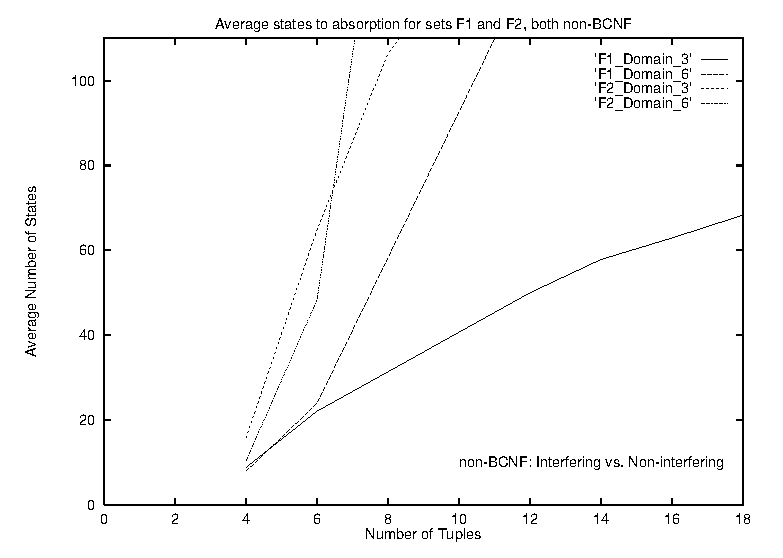
\includegraphics{../Evolve_papers/sets53_56.eps}}}
\caption{\label{graph:56_34}\scriptsize{Average states to absorption for sets $F_3$ and $F_4$, Domain sizes: 3, 6 }}
\end{figure}
 

Data mining tools require a {\em quality function} which assesses
and classifies the knowledge discovered in a form which is understandable
by the user \cite{hs94}. Our quality function describes the proximity of
relation $s$ to an Armstrong relation for FD set F, being one when the evolved 
example relation is an Armstrong relation. This was taken to be the
 symmetric difference of $GEN(F)$ and $GEN(dep(s))$, providing a direct ratio
 between the sets of generators, and is stated as:
\begin{displaymath}
quality(F, s) = \frac{\mid GEN(F) \cap GEN(dep(s)) \mid}{\mid GEN(F) \cup GEN(dep(s))\mid }
\end{displaymath}

\smallskip

\begin{figure}
\centerline{\scalebox{0.7}{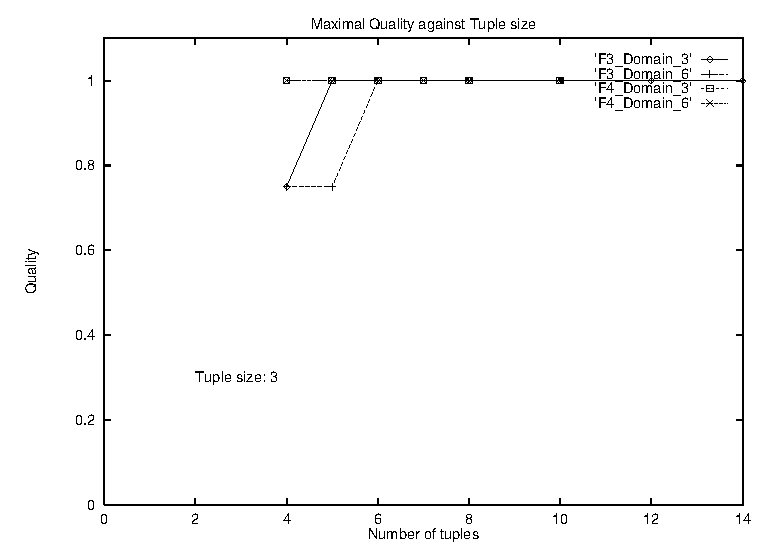
\includegraphics{../Evolve_papers/qsets28_t3.eps}}}
\caption{\label{graph:28_56}\scriptsize{Max Quality vs. Tuple size for FD sets  $F_3$ and $F_4$ }}
\end{figure}

Figure~\ref{graph:28_56} shows the maximal quality achieved within a 
batch for sets $F_3$ and $F_4$.  It is interesting that a maximal
quality of one for set $F_3$ is not one for a low tuple size (equal
to $\mid GEN(F) \mid$ when the domain is 3 and does not become one with
domain size 6 until the tuple size is 6. This is because the probability
of evolving an Armstrong relation is evidently lower when the tuple size
 is below
$\mid GEN(F) \mid + 1$. With a larger domain the chance of an example
relation being Armstrong is significantly lower, especially when the
domain and tuple sizes are comparable, often leading to a trivial
satisfaction of the FDs as well as FDs outside the specified set.
For an empty FD set over $R$ any random relation with schema $R$ satisfies this set;
in terms of quality every possible FD would need to be violated for such
a relation to be Armstrong.
 With a null FD set $\mid GEN(F) \mid = \mid R \mid$ and so
anything larger than a binary domain is unlikely to ever be an Armstrong
relation given the possible spread of all random relations. A measure
of the pathology of an FD set F can be
 provided by the ratio
of the determinations in F to the number of all possible determinations
which can occur over the schema $R$.
Given an attribute set and an FD set
which explicitly specifies all possible non-trivial FDs which
can hold amongst the attributes except for one FD then it is highly likely that
many relations will be evolved which in addition violate this FD. Thus within
such a batch it is likely that many example evolutions will be Armstrong
relations. The
pathology of FD sets has been examined and those which do not 
contain determinations between many of the attributes are
likely to have a lower proximity to an Armstrong relation; this does
not generally detract from their usefulness as example relations.

\medskip


We now
present some instructive examples for the set of FDs, $\{ AB \to D, 
BC \to D, D \to E, E \to A \}$, including an Armstrong relation
evolved with fewer tuples than what is capable using a 
deterministic algorithm. For a number of relations and FD sets,
including the example presented in Section~\ref{sec:intro}, it is often the
case that an Armstrong relation may be returned with fewer tuples than
the result of a deterministic generation.

\begin{example}
\begin{rm}
We show the result of forming an Armstrong relation (AR) for this set
in Table~\ref{table:5.1}, using Algorithm 14.2 in \cite{Mann92}. It has
7 tuples (exactly $\mid GEN(F) \mid + 1$) and a domain size of 5. If
 the values of each attribute domain are disjoint then the columns
of the example relations are disjoint; we therefore take the domain size
 for
the relation to be the maximal domain size in any one column. Table~\ref{table:5.2} depicts the final state of an evolutionary run applied to
this set of dependencies. It is an Armstrong relation but has only
six tuples and a domain size of 4. We can see that the probabilistic
process has resulted in a more compact relation which conveys the information
more succinctly to the database designer.  Table~\ref{table:5.3} presents
the best attained relation having only 4 tuples, less than the
minimum for evolving an Armstrong relation, with a quality of 0.7. Based on our
measure of quality this relation satisfies some dependencies outside of
the specified set, namely $\{ E \to D, D \to B \}$. Table~\ref{table:5.4} contains
a somewhat larger Armstrong relation with 9 tuples and a domain size 5.
\end{rm}
\end{example}

{\line
\begin{table}[ht]
\begin{minipage}[t]{8cm}
\begin{center}
\begin{tabular}{|c|c|c|c|c|} \hline 
{ \bf A } & { \bf B} & {\bf  C }  & { \bf D }  & {\bf E} \\ \hline
0 & 0 & 0 & 0 & 0 \\
1 & 0 & 1 & 1 & 1 \\
2 & 1 & 1 & 2 & 2 \\
2 & 2 & 1 & 3 & 3 \\
2 & 3 & 1 & 4 & 3 \\
2 & 3 & 2 & 4 & 3 \\
2 & 4 & 2 & 4 & 3 \\ \hline
\end{tabular}
\end{center}
\caption{\label{table:5.1} Standard AR}
\end{minipage}
\hfill
\begin{minipage}[t]{8cm}
\begin{center}
\begin{tabular}{|c|c|c|c|c|} \hline 
{ \bf A } & { \bf B} & {\bf  C }  & { \bf D }  & {\bf E} \\ \hline
1 & 0 & 3 & 0 & 0 \\
1 & 1 & 3 & 1 & 1 \\ 
1 & 2 & 3 & 2 & 0 \\
1 & 3 & 2 & 2 & 0 \\
1 & 3 & 3 & 2 & 0 \\
2 & 1 & 2 & 3 & 2 \\ \hline
\end{tabular}
\end{center}
\caption{\label{table:5.2} An evolved AR }
\end{minipage}
\end{table}
}

{\line
\begin{table}[ht]
\begin{minipage}[t]{8cm}
\begin{center}
\begin{tabular}{|c|c|c|c|c|} \hline 
{ \bf A } & { \bf B} & {\bf  C }  & { \bf D }  & {\bf E} \\ \hline
2 & 3 & 0 & 4 & 3 \\
4 & 1 & 0 & 1 & 1 \\
4 & 1 & 2 & 1 & 1 \\
4 & 3 & 2 & 0 & 4 \\  \hline
\end{tabular}
\end{center}
\caption{\label{table:5.3} Evolved relation }
\end{minipage}
\hfill
\begin{minipage}[t]{8cm}
\begin{center}
\begin{tabular}{|c|c|c|c|c|} \hline 
{ \bf A } & { \bf B} & {\bf  C }  & { \bf D }  & {\bf E} \\ \hline
0 & 1 & 2 & 4 & 0 \\
0 & 2 & 0 & 0 & 4 \\
0 & 4 & 0 & 4 & 0 \\
2 & 2 & 3 & 2 & 1 \\
3 & 0 & 1 & 3 & 2 \\
3 & 1 & 4 & 1 & 2 \\
3 & 2 & 1 & 1 & 2 \\
3 & 2 & 4 & 1 & 2 \\
3 & 3 & 2 & 1 & 2 \\ \hline\end{tabular}
\end{center}
\caption{\label{table:5.4} A larger AR }
\end{minipage}
\end{table}
}

The evolutionary procedure is now highlighted with some real world 
examples, with the intention of providing the reader with an 
appreciation of the utility of varied example relations. It
can be said that a greater understanding of the semantics of 
an FD set
is reached by repeated examinations of different instances of the
example relations; this is one motivating factor behind our probabilistic approach.

\begin{example}
\begin{rm}
We use the following non-BCNF FD set F =
$\{ Name \to Phone$ $Flat No.$, $Flat No. \to Name$, $Postcode \to City \}$.
Again we present a deterministic Armstrong relation for this set of 
dependencies together with three different evolved Armstrong relations
of varying tuple and domain size. Table~\ref{table:5.31} shows
an Armstrong relation evolved using a deterministic process and an evolved
Armstrong relation is shown in Table~\ref{table:5.32}. A quick
inspection of these two relations shows that the differences in
Armstrong relations with the same domain and tuple sizes tend to be
superficial, yet the stochastic nature of the generation of relations leads
 a more well-rounded view of the data. Tables~\ref{table:5.33}
and~\ref{table:5.34} contain two other Armstrong relations, the former 
extending the domain size of the deterministic Armstrong relation slightly and the latter
presenting an Armstrong relation with a domain size 8 and 9 tuples. In
this instance a larger relation highlights both the satisfied
and violated dependencies thoroughly. 
\end{rm}
\end{example}

{\line
\begin{table}[ht]
\begin{center}
\begin{tabular}{|c|c|c|c|c|} \hline 
{ \bf Name} & { \bf Phone} & {\bf Flat no. }  & { \bf Postcode}  & {\bf City} \\ \hline
Dave & 1246 & 19 & NW1 & London  \\
Dave & 1246 & 19 & YO2 & York \\
Dan & 3748 & 7 & YO2 & York \\
Dan & 3748 & 7 & YO1 & York \\
Charles & 3748 & 11 & YO1 & York \\ \hline
\end{tabular}
\end{center}
\caption{\label{table:5.31} Mannila's Armstrong relation for set 29 }
\end{table}
}

{\line
\begin{table}
\begin{center}
\begin{tabular}{|c|c|c|c|c|} \hline 
{ \bf Name} & { \bf Phone} & {\bf Flat no. }  & { \bf Postcode}  & {\bf City} \\ \hline
Dave & 1246 & 19 & NW1 & London  \\
Dave & 1246 & 19 & YO2 & York \\
Dan & 3748 & 7 & NW1 & London \\
Dan & 3748 & 7 & W14 & London \\
Charles & 1246 & 11 & YO2 & York \\ \hline
\end{tabular}
\end{center}
\caption{\label{table:5.32} An evolved AR with the same domain size }
\end{table}
}

{\line
\begin{table}[ht]
\begin{center}
\begin{tabular}{|c|c|c|c|c|} \hline 
{ \bf Name} & { \bf Phone} & {\bf Flat no. }  & { \bf Postcode}  & {\bf City} \\ \hline
Dave & 1246 & 19 & YO1 & York  \\
Dave & 1246 & 19 & NW1 & London \\
Dan & 1246 & 7 & W14 & London \\
Dan & 1246 & 7 & NW1 & London \\
Charles & 3748 & 11 & YO2 & York \\ \hline
\end{tabular}
\end{center}
\caption{\label{table:5.33} An AR with a larger domain size }
\end{table}
}

{\line
\begin{table}
\begin{center}
\begin{tabular}{|c|c|c|c|c|} \hline 
{ \bf Name} & { \bf Phone} & {\bf Flat no. }  & { \bf Postcode}  & {\bf City} \\ \hline
Dave & 1246 & 19 & NW1 & London  \\
Dave & 1246 & 19 & W14 & London \\
Dave & 1246 & 19 & YO3 & York \\
Dan & 1246 & 7 & BS8 & Bristol \\
Dan & 1246 & 7 & BA1 & Bath \\
Dan & 1246 & 7 & BA2 & Bath \\
Charles & 1246 & 11 & YO2 & York \\
Matt & 8881 & 84 & BA8 & Bath \\
Fred & 2383 & 24 & YO3 & York \\ \hline
\end{tabular}
\end{center}
\caption{\label{table:5.34} An evolved AR with 9 tuples }
\end{table}
}

\medskip

\begin{figure}
\centerline{\scalebox{0.7}{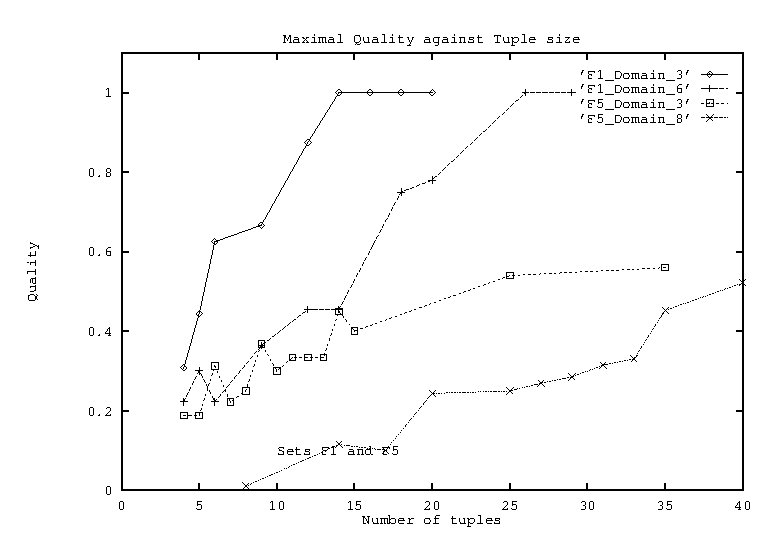
\includegraphics{../Evolve_papers/qsets93_t3.eps}}}
\caption{\label{graph:93_60}\scriptsize{Max Quality vs. Tuple size for FD sets $F_1$ and $F_5$ }}
\end{figure}

We now move on to examine the pathological sets, these being
the sets for which an Armstrong relation was only rarely,
or in some cases never, achieved. Pathological sets are
defined as sets which contain attributes in the schema with none or
few
determinations specified in the FD set; they are more likely,
though not necessarily, to have a large $\mid GEN(F) \mid$. One
such set which is unlikely to have a high quality is the null
set of FDs. An example of sets which have an exponential $\mid GEN(F) \mid$
in the size of the FD set are discussed in \cite{bdfs84}.
These sets possess the following pattern: $\{ A_1A_2 \to B, A_3A_4 \to B, \ldots , A_{2m-1}A_{2m} \to B \}$ which has  $\mid GEN(F) \mid = 2^m$ and for
our simulations resulted in examples with a low proximity to Armstrong.
To exemplify why, any possible relationship between $A_i$ and $A_j, i \not= j$ is not discouraged. Larger attribute combination sets are also
unlikely to be violated for anything above a binary domain, such as
$A_5A_3 \to A_1A_2A_6$, where there is little chance of repititions
within either the left or right hand sides.
As we have noted
our procedure only evolves relations by mutating attributes of FDs which are
inside the specified set and not by forcing violations of FDs which hold outside of the specified set. 
Figure~\ref{graph:93_60} highlights the maximal qualities achieved for
two FD sets, $F_1$, as detailed earlier, and $F_5$ = $\{ AB \to G, CD \to G,
EF \to G \}$; $F_5$ following the form of the FD sets described previously
and in \cite{bdfs84}.  For $F_5$ there are many attributes which
are independent of each other and so it is highly improbable that an 
Armstrong relation will be formed. It is also interesting to note that
the best results, in terms of proximity to Armstrong, may be achieved 
with a lower domain size and more tuples  (the best evolution had a domain size of 3 and 35 tuples) than what would be incorporated
into a deterministic generation of the same FD set (requiring 15 tuples
and domain size 9).

\medskip

For pathological sets an Armstrong relation could be evolved with
a higher probability if the number 
of tuples were initially much larger than the number of elements in $GEN(F)$
and the domain size were small, as the likelihood of providing counterexamples
within such an example increases.
A better technique, however, would be to incorporate a penalising
procedure which violates dependencies that hold in a relation but which are
outside of the specified set. Based upon the results of our simulations we
conclude that the use of this could be restricted to when
a dependency set has a large $\mid GEN(F) \mid$. In instances when
an Armstrong relation is not achievable, either due to a domain or
tuple size deficiency, then a limit would have to be placed on iterating
between violating unwanted FDs and satisfying desired FDs, so as to
avoid infinite loops.
Another option is that for any FD set F and final relation state our counterexample
procedure to violate extraneous FDs can be used
to extend any example relation with counterexamples, one at a time, for all of the FDs which are not violated.
Alternatively, we can extend our example relation with counterexamples, one
at a time, for all extraneous FDs that are not violated within the relation.
\medskip

To conclude, the results have shown that example relations which satisfy sets
of FDs can be efficiently evolved. The many different
relations which can be studied for the same FD set also provide a
more well-rounded view of the data in the designer's mind.
Batches containing
many evolutions can be run and a database designer would then be able
to view many relations, including those that are Armstrong if the domain
and tuple sizes satisfy the size bounds and an Armstrong relation
was actually evolved.  If they do not, either domain
or tuple size being too low, then the designer can view an
approximation to an Armstrong which a batch has provided. In
non-pathological cases it is likely that
this will be the best, or close to the best, approximation to Armstrong
which exists.

\smallskip

 Another extension of the 
design process is using our program as part of an evolving design
stage where relations which satisfy a dependency set but are not
Armstrong relations can be contrasted with Armstrong relations for
the same set and any 
additional dependencies which hold in the initial relation can
be studied to decide if the designer wishes these to be part
of the final schema. Such information might not be discovered without
different example relations and forms an interactive database design
process.



\section{Armstrong Relations for NDs}


\section{Discussion}



For design purposes the evolution of example relations has been shown to
be a useful tool.  A good database
design tool is based on ease of use for the designer and example relations
are a step in this direction.  To  study the applicability of a set of FDs
 the user can limit the number of tuples in
a relation as well as the domain size. The simulations have shown that 
informative example relations can be evolved by our process.  The 
average number of states to evolution is dependent on both
the nature (non-interfering or interfering) and size of the FD set and the size of the relation.
Example relations containing attributes independent of each other
are less likely to be evolved into Armstrong relations. For 63 out
of our 72 sets of FDs tested an Armstrong relation was evolved
for some domain/tuple combination; this is an important side-effect
of our approach and may form the basis for further research.\\

This work
will be of use to the database designer as an auxiliary tool to complement
the other stages of the design process.  From a schema the designer is now
 able to evolve many varied example relations.\\

